\documentclass{beamer}
\mode<presentation>{\usecolortheme{crane}}
\usetheme{Madrid}


\usepackage{graphicx}
\usepackage[utf8]{inputenc}
\usepackage{hyperref}
\hypersetup{
    colorlinks=true,
    linkcolor=blue,
    filecolor=magenta,
    urlcolor=cyan,
}

\title{CS633 Project: Parallel Debugger}
\author[Milind, Subhdeep]{Milind Luthra (150363) \and Subhdeep Saha (150732)}

\date{15 March 2019}

\AtBeginSection[]
{
  \begin{frame}{Table of Contents}
    \tableofcontents[currentsection]
  \end{frame}
}

\AtBeginSubsection[]
{
  \begin{frame}{Table of Contents}
    \tableofcontents[currentsubsection]
  \end{frame}
}

\begin{document}

\frame{\titlepage}

\section{Overview}

\subsection{Motivation}
\begin{frame}
  \frametitle{Motivation}
  \begin{center}
      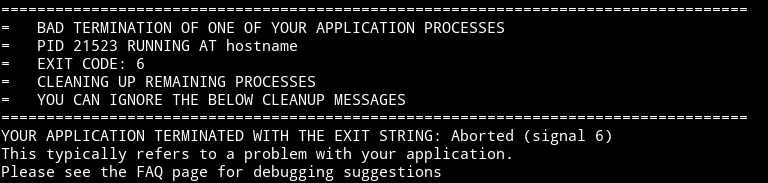
\includegraphics[width=0.9\textwidth]{motivation}
  \end{center}
\end{frame}

\subsection{Related Work}

\begin{frame}
  \frametitle{Allinea DDT and Totalview}
  \begin{itemize}
  \item <1-> Debuggers already in use to debug large parallel applications.
  \item <2-> Both have a rich feature set and GUIs.
  \item <3-> However, both are proprietary, commercial software.
  \item <5-> Restrictive licenses (locked to one node, or four processes etc) and high cost (a few hundred dollars).
  \item <6-> Can't be extended any further.
  \end{itemize}
\end{frame}

\begin{frame}[fragile]
  \frametitle{Using XTerm and GDB}
  \begin{itemize}
  \item <1-> Possible Idea: For n processes, launching n XTerm instances with gdb.
  \item <2-> Each terminal can be used to debug the individual processes.
  \item <3-> \texttt{mpiexec -n 4 xterm -e gdb ./test}
  \end{itemize}
\end{frame}

\begin{frame}
  \frametitle{Problems with XTerm + GDB}
  \texttt{mpiexec -n 30 xterm -e gdb ./test}

  \begin{center}
    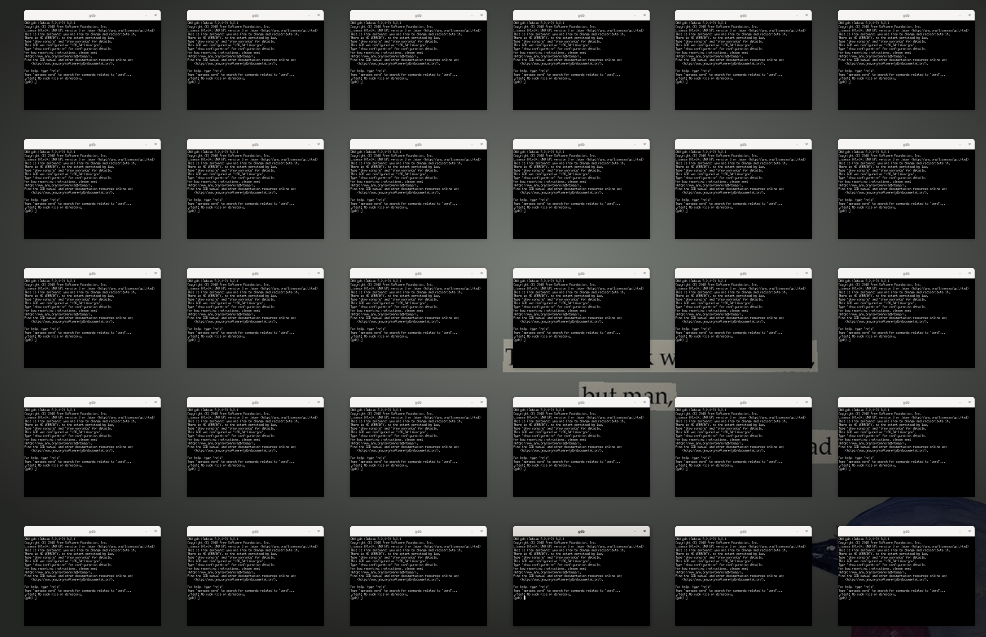
\includegraphics[width=0.9\textwidth]{usingxterm}
  \end{center}
\end{frame}


\subsection{Idea}
\begin{frame}
  \frametitle{Basic Idea}
\begin{itemize}
  \item <1-> The basic idea is to launch a number of clients on nodes using \texttt{mpiexec}.
  \item <2-> Each client instance will run a \texttt{gdb} instance with the program to be debugged.
  \item <3-> All the instances of \texttt{gdb} are controlled using a single, centralized interface.
\end{itemize}
\end{frame}

\begin{frame}
  \frametitle{Basic Idea}
  \begin{center}
   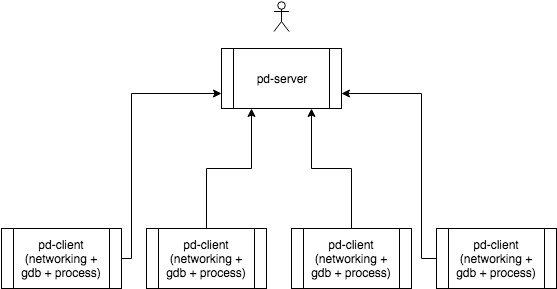
\includegraphics[width=0.8\textwidth]{flow}
  \end{center}
\end{frame}
\section{Implementation}
\subsection{parallel-debugger-client (pd-client)}

\begin{frame}
  \frametitle{pd-client}
  \begin{itemize}
  \item <1-> Handles the networking of an individual client to the server.
    \begin{itemize}
      \item <2-> Sends request to the server using \textbf{TCP sockets}.
    \end{itemize}
    \item  <3-> Loads the target binary \texttt{./test} and instrument it using
    LD preload.
  \item <4-> Acts as a frontend to the GDB interpreter \texttt{mi2}.
    \begin{itemize}
    \item <5-> Conveys the instructions from the server to individual clients.
    \end{itemize}
  \end{itemize}
\end{frame}

\begin{frame}
  \frametitle{Machine Interface (mi)}
  \begin{itemize}
  \item <1-> {Currently GDB supports multiple command interpreters, and
      some of them are used to make user interface for the GDB}
  \item <2-> {\textbf{mi2} is a line based machine oriented text interface to
    GDB}
\item <3-> {The default interpreter is the \textbf{Console Interpreter}. For
   a different interpreter user can use}
\item <3-> {\texttt{gdb .test --interpreter=(console|mi|mi2)}}
\end{itemize}
\end{frame}

\begin{frame}
  \frametitle{mi2 vs console}
  \begin{columns}
      \begin{column}{0.5\textwidth}
        \begin{center}
          \textbf{mi2}
          \end{center}
    \begin{itemize}
      \item <1-> \texttt{-file-exec-and-symbols ./test}
      \item <2-> \texttt{-break-insert main}
      \item <3-> \texttt{-exec-run}
      \item <4-> \texttt{-exec-continue}
      \end{itemize}
    \end{column}
    \begin{column}{0.5\textwidth}
      \begin{center}
        \textbf{console}
      \end{center}
      \begin{itemize}
      \item <1-> \texttt{file ./test}
      \item <2-> \texttt{break main}
      \item <3-> \texttt{run}
      \item <4-> \texttt{continue}
      \end{itemize}
    \end{column}
  \end{columns}
\end{frame}

\subsection{parallel-debugger-server (pd-server)}

\begin{frame}
  \begin{itemize}
  \item <1-> Ensures that all the clients are connected to it.
  \item <2-> Maintains a in-memory \texttt{map[rank int]conn *net.Conn} to store the clients that are already
    connected.
  \end{itemize}
  \frametitle{pd-server}
\end{frame}

\section{Features}

\subsection{General Debugging Features}

\begin{frame}
  \frametitle{General Debugging Features}
 \begin{itemize}
 \item <1-> The main feature is to expose all the power of gdb in a user-friendly way (through a TUI).
 \item <2-> Example: Set a breakpoint on \texttt{MPI\_Allgather} in \textit{each} process.
 \item <3-> \texttt{(pdb) break MPI\_Allgather}
 \item <4-> Example: Selectively print \texttt{argc} in processes with rank 4, 5, 6 (with respect to MPI\_COMM\_WORLD).
 \item <5-> \texttt{(pdb) pdb\_print argc [r=4,5,6]}
 \end{itemize}
\end{frame}

\begin{frame}
  \frametitle{General Debugging Features}
 \begin{itemize}
 \item <1-> Example: List all communicators and associated processes' rank.
 \item <2-> \texttt{(pdb) pdb\_listcomm}
 \item <3-> Example: Selectively set breakpoint in processes in communicator 4.
 \item <4-> \texttt{(pdb) pdb\_break MPI\_Allgather [c=4]}
 \end{itemize}
\end{frame}


\subsection{MPI Specific Features}
\begin{frame}
  \frametitle{Missing Collective Calls}
 \begin{itemize}
 \item <1-> Missing a collective call in any one process of a communicator is a source of errors.
 \item <2-> We are maintaining a communicator to processes mapping.
 \item <3-> We can use this to maintain a list of collectives pending on a process.
 \item <4-> Example: Listing all pending collectives.
 \item <5-> \texttt{(pdb) pdb\_listcoll}
 \end{itemize}
\end{frame}

\begin{frame}
  \frametitle{Modifying Buffer During Asynchronous Calls}
 \begin{itemize}
 \item <1-> A buffer passed to \texttt{MPI\_Isend} cannot be written to until we're sure that the it has been copied.
 \item <2-> Usually done using \texttt{MPI\_Wait} or \texttt{MPI\_Test}.
 \item <3-> We can track asynchronous calls using breakpoints.
 \item <4-> We can track buffer writes using watchpoints.
 \item <5-> Hence, we can give feedback for any invalid write.
 \end{itemize}
\end{frame}

\section{Timeline}
\begin{frame}
  \frametitle{Timeline}
  \begin{itemize}
  \item <1-> Load and then instrument target binary in all nodes. \textsc{Done}
  \item <2-> Communicate with \texttt{gdb/mi}. \textsc{Done}
  \item <3-> Set up client and server communication (extract rank/size from instrumented binary). \textsc{Done}
  \item <4-> Allow commands from server to all clients, and echo client console on server. \textsc{Done}
  \end{itemize}
\end{frame}

\begin{frame}
  \frametitle{Timeline}
  \begin{itemize}
  \item <1-> Allow sending commands from server to only specific clients \textsc{Todo}
  \item <2-> Make a nice TUI. \textsc{Todo}
  \item <3-> Track communicator data and collective calls. \textsc{IfPossible}
  \item <4-> Track asynchronous call buffers. \textsc{IfPossible}
  \item <4-> Make a nice GUI. \textsc{IfAnyoneVolunteers}
  \end{itemize}
\end{frame}

\section{References}
\begin{frame}
  \frametitle{References}
  \begin{itemize}
  \item \href{https://sourceware.org/gdb/onlinedocs/gdb/GDB_002fMI.html}{GDB/MI2 Documentation}
  \item \href{https://github.com/cyrus-and/gdb}{Go library for talking to GDB/MI} - \href{https://github.com/milindl/gdb}{Our modified version of the library}.
  \item \href{https://en.wikipedia.org/wiki/Allinea_DDT}{Allinea DDT}, \href{https://www.roguewave.com/products-services/totalview}{TotalView}
  \item \href{https://www.open-mpi.org/faq/?category=debugging}{OpenMPI FAQ for Parallel Debugging}
  \item \href{http://www.linux-mag.com/id/7210/}{Common MPI Programming Errors}
  \end{itemize}
\end{frame}

\end{document}